\chapter{Control, Simulation \& Visualization}
\label{ch:software}

The Eelume robot is controlled using a low-level \gls{api} that Eelume AS made
available in the beginning of 2025.
This \gls{api} privides access to an internal \gls{can} bus, which is used to
communicate with the robot's thrusters, joints, and sensors. The \gls{api} provides
a set of functions for packaging and unpacking messages to and from the bus, giving
access to functions for generating, for example, thruster force references and
joint torque references.
The \gls{api} is implemented in C/C++ and communicates with the robot over
an ethernet connection. Because the \gls{api} is low-level, a lot of code had
to be written to implement the \gls{tpc} framework, everything from
lower-level controllers, task definitions, and kinematics. The collection of
code used to control the Eelume robot is created as a C++ library
and is refered to as \gls{eck}.

The control kit is designed to be modular, allowing for easy integration of
new tasks and controllers. The library provides a set of virtual base classes,
one for a controller and one for a connection to the Eelume robot, along with
a set of concrete implementations for these classes. Setting and reading data
from the robot is done through the \gls{api} using a connection class, while 
a simulator is also provided for testing the controllers without the need for
a physical robot. Lower-level \gls{dp} controllers, as well as higher-level
\gls{tpc}lers are also implemented.

The simulator is designed to mimic the behavior of the Eelume robot as closely
as possible, without much time spent on modeling the hydrodynamics and coupling
between the links. The kinematics of the robot is thought to be accurately
implemented. Because of the virtual base classes, the real robot can be used
interchangeably without recompiling the code. This allows for easy testing of
the controllers after verifying that they work in the simulator.

In addition to the control kit, the need for visualization of the robot and
the tasks was identified. A simple visualizer was created to display the robot
in real time as experiments are conducted. The visualizer is implemented in
C++ using the OpenGL graphics library. The control kit communicates with the
visualizer over \gls{udp} sockets, sending the robot's state and task definitions.

All figures of the Eelume robot within this thesis have been created using this visualizer.

An example of the visualizer as it is used during experiments is shown in
\autoref{fig:eelume:visualizer}. One can see gridlines in the background, and
an axis system in the center showing the \gls{ned} frame origin.
\begin{figure}[h!]
    \centering
    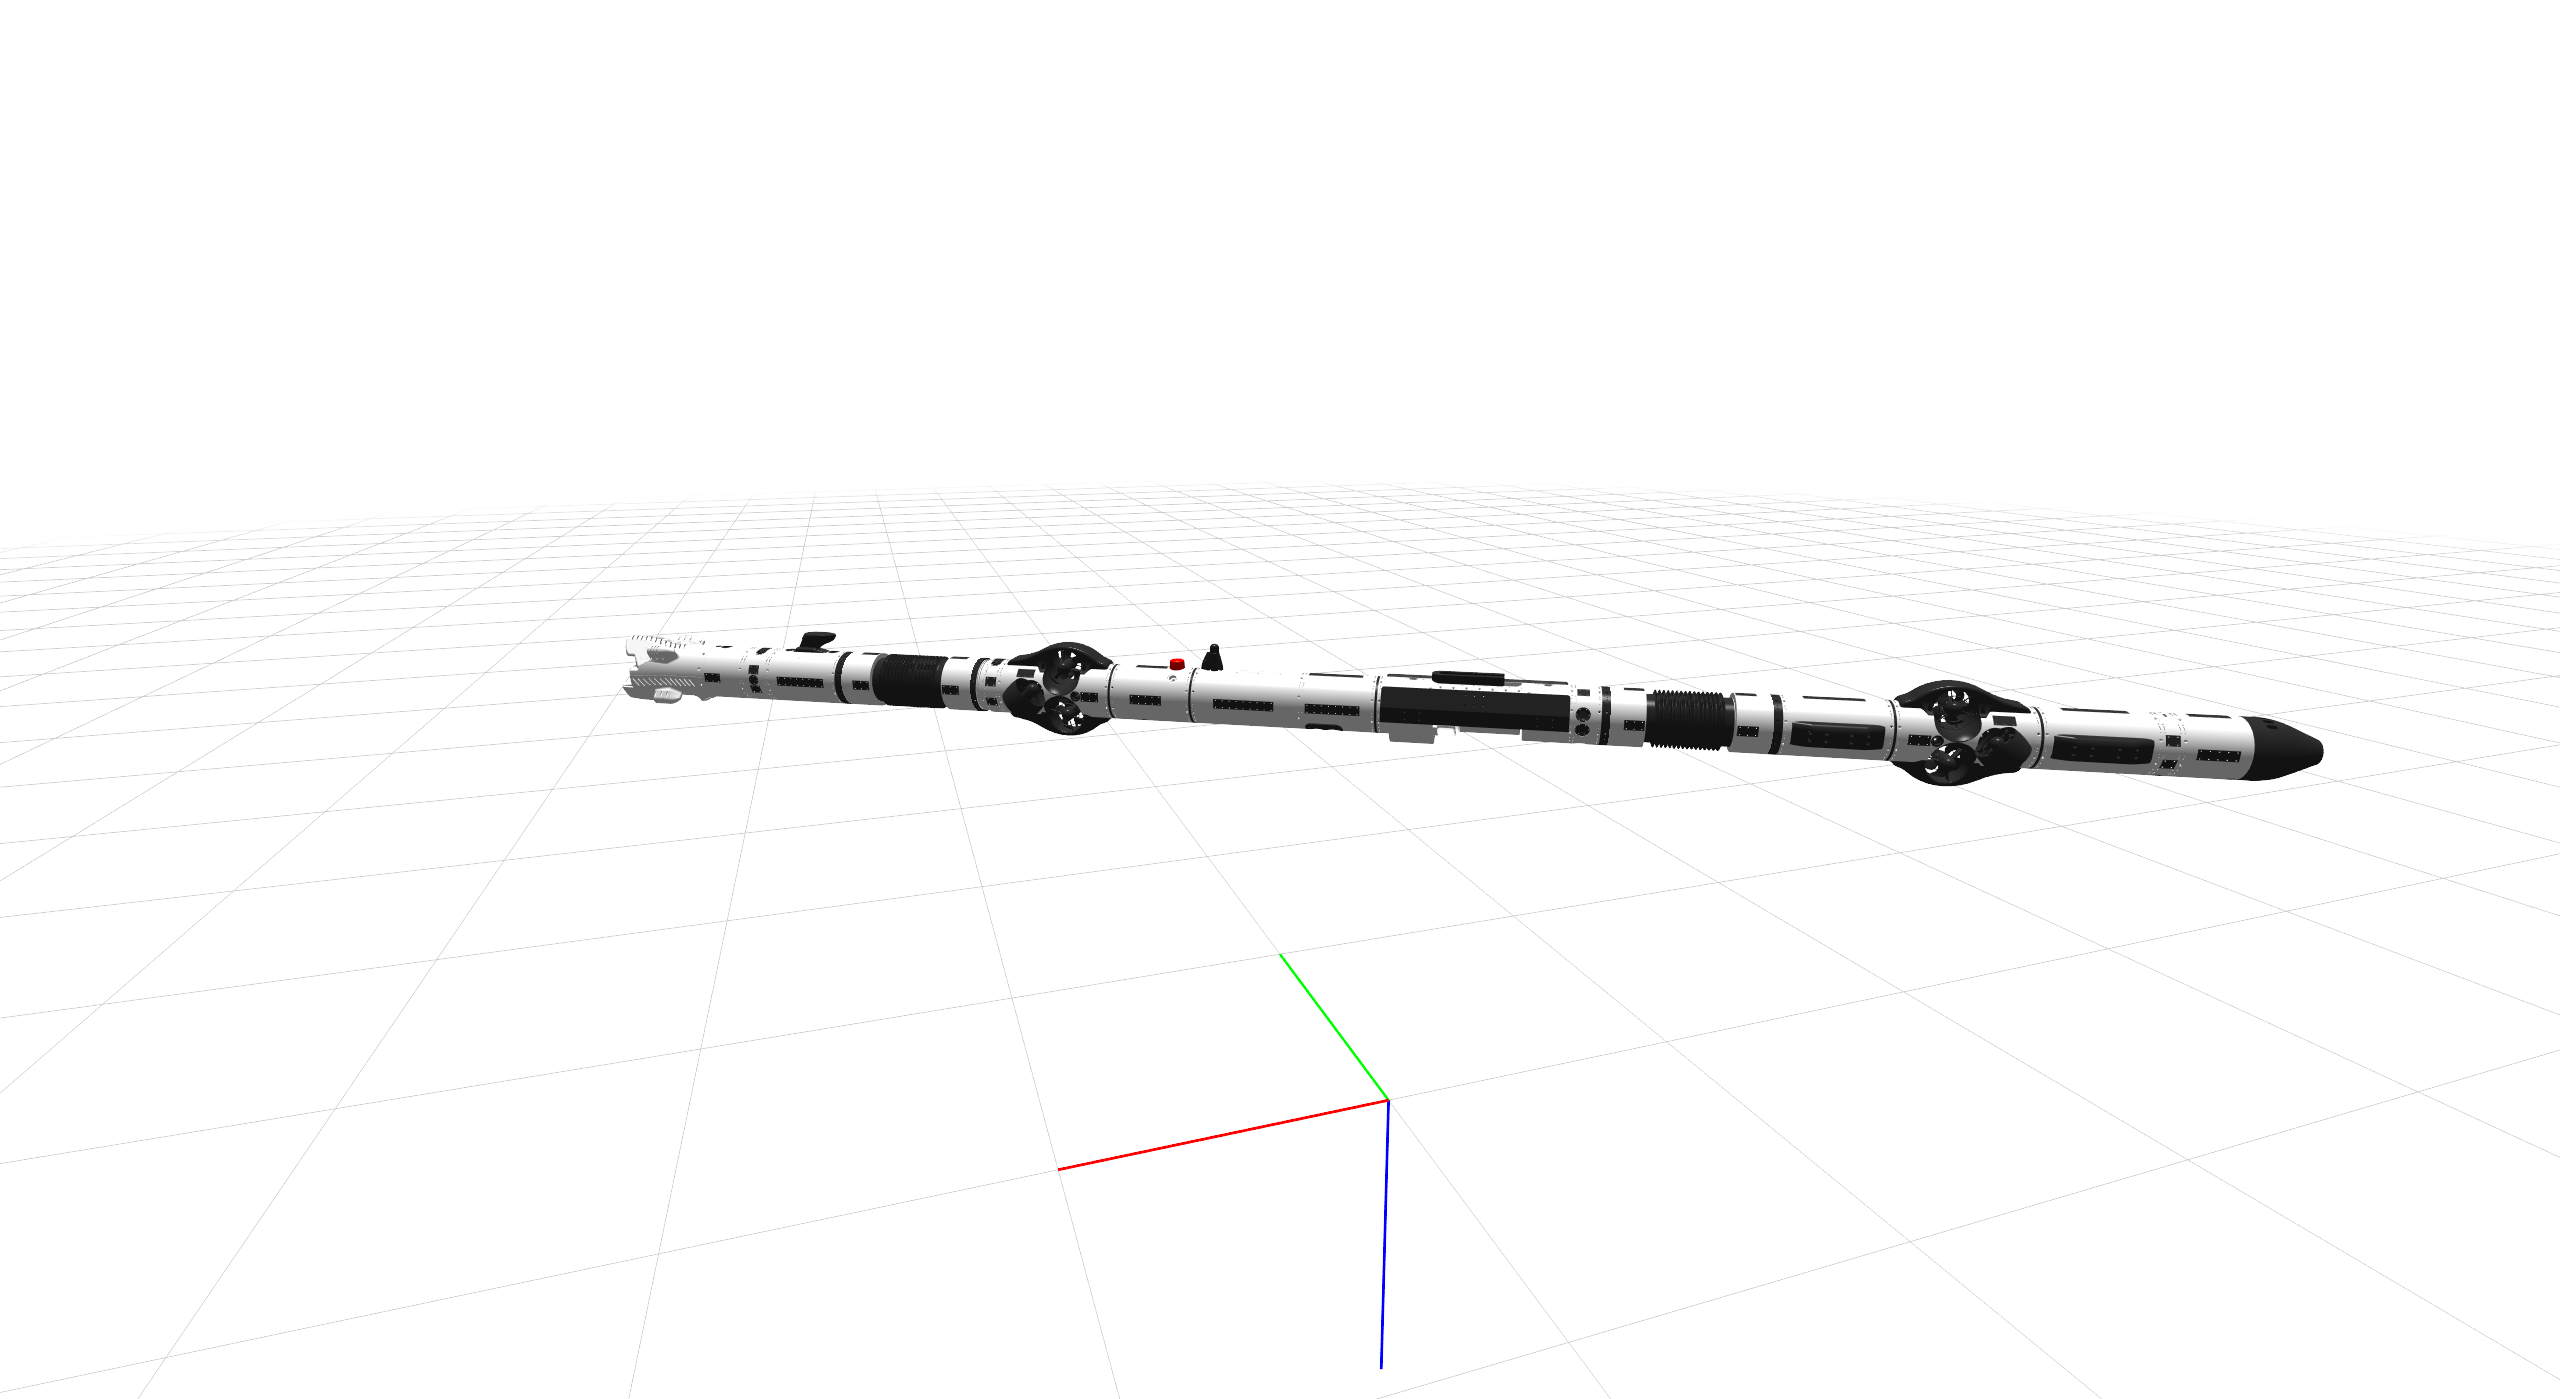
\includegraphics[width=\textwidth]{assets/eely-visualizer.png}
    \caption{A screenshot of the Eelume visualizer.}
    \label{fig:eelume:visualizer}
\end{figure}


\section{EelyControlKit}
\section{Simulator}
\section{Visualizer}

